\documentclass{standalone}
\usepackage{tikz}
\usetikzlibrary{patterns, positioning}
\usepackage[sfdefault]{ClearSans} %% option 'sfdefault' activates Clear Sans as the default text font
\usepackage[T1]{fontenc}

\begin{document}
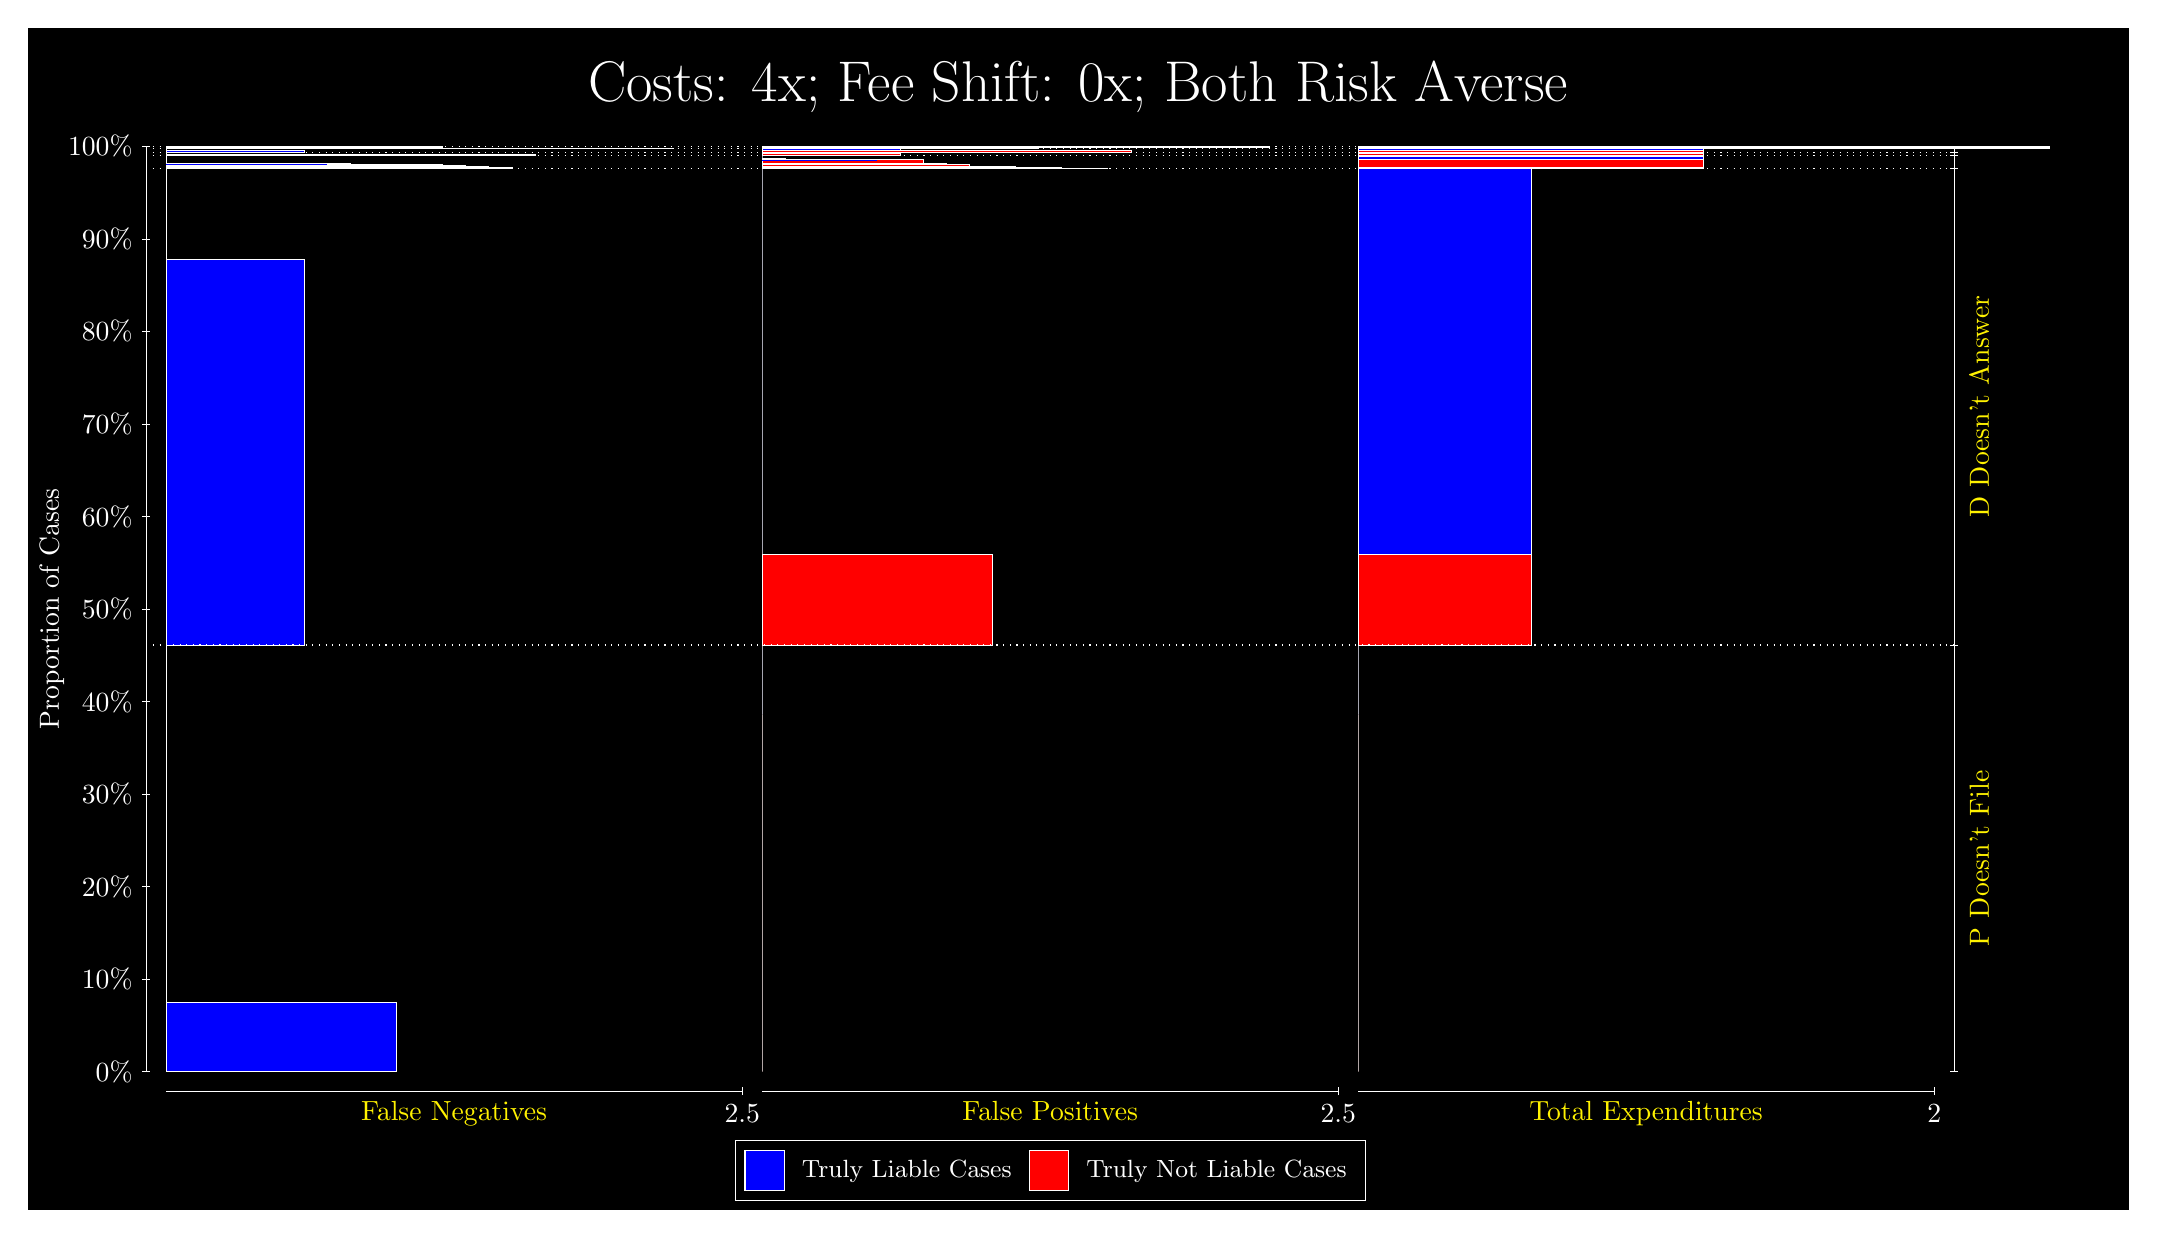
\begin{tikzpicture}
\draw[fill=black] (0,0) rectangle (26.667,15);
\draw[text=white] (0,13.5) rectangle (26.667,15) node[midway] {\huge Costs: 4x; Fee Shift: 0x; Both Risk Averse};
\draw[white, very thin] (1.5,1.75) -- (1.5,13.5);
\node[rotate=90, text=white, anchor=center] at (0.3, 7.625) {Proportion of Cases};
\draw[white, very thin] (1.45,1.75) -- (1.55,1.75);
\node[text=white, anchor=east] at (1.45, 1.75) {0\%};
\draw[white, very thin] (1.45,2.925) -- (1.55,2.925);
\node[text=white, anchor=east] at (1.45, 2.925) {10\%};
\draw[white, very thin] (1.45,4.1) -- (1.55,4.1);
\node[text=white, anchor=east] at (1.45, 4.1) {20\%};
\draw[white, very thin] (1.45,5.275) -- (1.55,5.275);
\node[text=white, anchor=east] at (1.45, 5.275) {30\%};
\draw[white, very thin] (1.45,6.45) -- (1.55,6.45);
\node[text=white, anchor=east] at (1.45, 6.45) {40\%};
\draw[white, very thin] (1.45,7.625) -- (1.55,7.625);
\node[text=white, anchor=east] at (1.45, 7.625) {50\%};
\draw[white, very thin] (1.45,8.8) -- (1.55,8.8);
\node[text=white, anchor=east] at (1.45, 8.8) {60\%};
\draw[white, very thin] (1.45,9.975) -- (1.55,9.975);
\node[text=white, anchor=east] at (1.45, 9.975) {70\%};
\draw[white, very thin] (1.45,11.15) -- (1.55,11.15);
\node[text=white, anchor=east] at (1.45, 11.15) {80\%};
\draw[white, very thin] (1.45,12.325) -- (1.55,12.325);
\node[text=white, anchor=east] at (1.45, 12.325) {90\%};
\draw[white, very thin] (1.45,13.5) -- (1.55,13.5);
\node[text=white, anchor=east] at (1.45, 13.5) {100\%};

\draw[white, very thin] (24.457,1.75) -- (24.457,13.5);
\draw[white, very thin] (24.407,1.75) -- (24.507,1.75);
\node[anchor=west] at (24.407, 1.75) {};
\draw[white, very thin] (24.407,7.1668) -- (24.507,7.1668);
\node[anchor=west] at (24.407, 7.1668) {};
\draw[white, very thin] (24.407,13.222) -- (24.507,13.222);
\node[anchor=west] at (24.407, 13.222) {};
\draw[white, very thin] (24.407,13.389) -- (24.507,13.389);
\node[anchor=west] at (24.407, 13.389) {};
\draw[white, very thin] (24.407,13.424) -- (24.507,13.424);
\node[anchor=west] at (24.407, 13.424) {};
\draw[white, very thin] (24.407,13.472) -- (24.507,13.472);
\node[anchor=west] at (24.407, 13.472) {};
\draw[white, very thin] (24.407,13.493) -- (24.507,13.493);
\node[anchor=west] at (24.407, 13.493) {};
\draw[white, very thin] (24.407,13.5) -- (24.507,13.5);
\node[anchor=west] at (24.407, 13.5) {};

\draw[white, very thin, fill=blue] (1.75,1.75) rectangle (4.6775,2.6306);
\draw[white, very thin, fill=red] (1.75,2.6306) rectangle (1.75,7.1668);
\draw[white, very thin, fill=blue] (1.75,7.1668) rectangle (3.5065,12.065);
\draw[white, very thin, fill=red] (1.75,12.065) rectangle (1.75,13.222);
\draw[white, very thin, fill=blue] (1.75,13.222) rectangle (6.1413,13.239);
\draw[white, very thin, fill=blue] (1.75,13.239) rectangle (5.8486,13.252);
\draw[white, very thin, fill=blue] (1.75,13.252) rectangle (5.5558,13.26);
\draw[white, very thin, fill=blue] (1.75,13.26) rectangle (5.2631,13.266);
\draw[white, very thin, fill=blue] (1.75,13.266) rectangle (4.9703,13.272);
\draw[white, very thin, fill=blue] (1.75,13.272) rectangle (4.6775,13.275);
\draw[white, very thin, fill=blue] (1.75,13.275) rectangle (4.3848,13.278);
\draw[white, very thin, fill=blue] (1.75,13.278) rectangle (4.092,13.28);
\draw[white, very thin, fill=blue] (1.75,13.28) rectangle (3.7993,13.281);
\draw[white, very thin, fill=red] (1.75,13.281) rectangle (1.75,13.389);
\draw[white, very thin, fill=blue] (1.75,13.389) rectangle (6.4341,13.398);
\draw[white, very thin, fill=red] (1.75,13.398) rectangle (1.75,13.424);
\draw[white, very thin, fill=blue] (1.75,13.424) rectangle (3.5065,13.445);
\draw[white, very thin, fill=red] (1.75,13.445) rectangle (1.75,13.472);
\draw[white, very thin, fill=blue] (1.75,13.472) rectangle (8.1906,13.477);
\draw[white, very thin, fill=red] (1.75,13.477) rectangle (1.75,13.493);
\draw[white, very thin, fill=blue] (1.75,13.493) rectangle (5.2631,13.497);
\draw[white, very thin, fill=red] (1.75,13.497) rectangle (1.75,13.5);
\draw[white, very thin, fill=red] (9.3189,1.75) rectangle (9.3189,6.2862);
\draw[white, very thin, fill=blue] (9.3189,6.2862) rectangle (9.3189,7.1668);
\draw[white, very thin, fill=red] (9.3189,7.1668) rectangle (12.246,8.3245);
\draw[white, very thin, fill=blue] (9.3189,8.3245) rectangle (9.3189,13.222);
\draw[white, very thin, fill=red] (9.3189,13.222) rectangle (13.71,13.223);
\draw[white, very thin, fill=red] (9.3189,13.223) rectangle (13.417,13.225);
\draw[white, very thin, fill=red] (9.3189,13.225) rectangle (13.125,13.229);
\draw[white, very thin, fill=red] (9.3189,13.229) rectangle (12.832,13.233);
\draw[white, very thin, fill=red] (9.3189,13.233) rectangle (12.539,13.244);
\draw[white, very thin, fill=red] (9.3189,13.244) rectangle (12.246,13.252);
\draw[white, very thin, fill=red] (9.3189,13.252) rectangle (11.954,13.267);
\draw[white, very thin, fill=red] (9.3189,13.267) rectangle (11.661,13.29);
\draw[white, very thin, fill=red] (9.3189,13.29) rectangle (11.368,13.33);
\draw[white, very thin, fill=blue] (9.3189,13.33) rectangle (10.783,13.331);
\draw[white, very thin, fill=blue] (9.3189,13.331) rectangle (10.49,13.333);
\draw[white, very thin, fill=blue] (9.3189,13.333) rectangle (10.197,13.336);
\draw[white, very thin, fill=blue] (9.3189,13.336) rectangle (9.9044,13.339);
\draw[white, very thin, fill=blue] (9.3189,13.339) rectangle (9.6116,13.346);
\draw[white, very thin, fill=blue] (9.3189,13.346) rectangle (9.3189,13.389);
\draw[white, very thin, fill=red] (9.3189,13.389) rectangle (11.075,13.415);
\draw[white, very thin, fill=blue] (9.3189,13.415) rectangle (9.3189,13.424);
\draw[white, very thin, fill=red] (9.3189,13.424) rectangle (14.003,13.452);
\draw[white, very thin, fill=blue] (9.3189,13.452) rectangle (11.075,13.472);
\draw[white, very thin, fill=red] (9.3189,13.472) rectangle (12.832,13.489);
\draw[white, very thin, fill=blue] (9.3189,13.489) rectangle (9.9044,13.493);
\draw[white, very thin, fill=red] (9.3189,13.493) rectangle (15.759,13.496);
\draw[white, very thin, fill=blue] (9.3189,13.496) rectangle (12.832,13.5);
\draw[white, very thin, fill=red] (16.888,1.75) rectangle (16.888,6.2862);
\draw[white, very thin, fill=blue] (16.888,6.2862) rectangle (16.888,7.1668);
\draw[white, very thin, fill=red] (16.888,7.1668) rectangle (19.083,8.3245);
\draw[white, very thin, fill=blue] (16.888,8.3245) rectangle (19.083,13.222);
\draw[white, very thin, fill=red] (16.888,13.222) rectangle (21.279,13.233);
\draw[white, very thin, fill=blue] (16.888,13.233) rectangle (21.279,13.239);
\draw[white, very thin, fill=red] (16.888,13.239) rectangle (21.279,13.331);
\draw[white, very thin, fill=blue] (16.888,13.331) rectangle (21.279,13.379);
\draw[white, very thin, fill=red] (16.888,13.379) rectangle (21.279,13.384);
\draw[white, very thin, fill=blue] (16.888,13.384) rectangle (21.279,13.389);
\draw[white, very thin, fill=red] (16.888,13.389) rectangle (21.279,13.415);
\draw[white, very thin, fill=blue] (16.888,13.415) rectangle (21.279,13.424);
\draw[white, very thin, fill=red] (16.888,13.424) rectangle (21.279,13.452);
\draw[white, very thin, fill=blue] (16.888,13.452) rectangle (21.279,13.472);
\draw[white, very thin, fill=red] (16.888,13.472) rectangle (25.67,13.489);
\draw[white, very thin, fill=blue] (16.888,13.489) rectangle (25.67,13.493);
\draw[white, very thin, fill=red] (16.888,13.493) rectangle (25.67,13.496);
\draw[white, very thin, fill=blue] (16.888,13.496) rectangle (25.67,13.5);
\draw[white, dotted] (1.5,7.1668) -- (24.457,7.1668);
\draw[white, dotted] (1.5,13.222) -- (24.457,13.222);
\draw[white, dotted] (1.5,13.389) -- (24.457,13.389);
\draw[white, dotted] (1.5,13.424) -- (24.457,13.424);
\draw[white, dotted] (1.5,13.472) -- (24.457,13.472);
\draw[white, dotted] (1.5,13.493) -- (24.457,13.493);
\draw[white, very thin] (1.75,1.5) -- (9.0689,1.5);
\node[text=yellow, anchor=north] at (5.4094, 1.5) {False Negatives};
\draw[white, very thin] (9.0689,1.45) -- (9.0689,1.55);
\node[text=white, anchor=north] at (9.0689, 1.45) {2.5};

\draw[white, very thin] (9.3189,1.5) -- (16.638,1.5);
\node[text=yellow, anchor=north] at (12.978, 1.5) {False Positives};
\draw[white, very thin] (16.638,1.45) -- (16.638,1.55);
\node[text=white, anchor=north] at (16.638, 1.45) {2.5};

\draw[white, very thin] (16.888,1.5) -- (24.207,1.5);
\node[text=yellow, anchor=north] at (20.547, 1.5) {Total Expenditures};
\draw[white, very thin] (24.207,1.45) -- (24.207,1.55);
\node[text=white, anchor=north] at (24.207, 1.45) {2};

\node[text=yellow, centered, rotate=90] at (24.777, 4.4584) {P Doesn't File};
\node[text=yellow, centered, rotate=90] at (24.777, 10.195) {D Doesn't Answer};






\draw (12.978300999999998,1.5) node[draw=none] (baseCoordinate) {};
\begin{scope}[align=center]
        \matrix[scale=0.5, draw=white, below=0.5cm of baseCoordinate, nodes={draw}, column sep=0.1cm]{
            \node[rectangle, draw, minimum width=0.5cm, minimum height=0.5cm, fill=blue] {}; &
            \node[draw=none, font=\small, text=white] (B) {Truly Liable Cases}; &
            \node[rectangle, draw, minimum width=0.5cm, minimum height=0.5cm, fill=red] {}; &
            \node[draw=none, font=\small, text=white] (B) {Truly Not Liable Cases}; \\
            };
\end{scope}

\end{tikzpicture}
\end{document}